%Encoding utf8
%Author:    Pavol Loffay, xloffa00
%           Miroslav Lisik, xlisik00
%           Dušan Maďarka, xmadar00
%           Fridolín Pokorný, xpokor32
%Date:2.10.2011



\documentclass[11pt,a4paper,titlepage]{article}

\usepackage[slovak]{babel}
\usepackage[top=3.0cm, left=2.0cm, text={17cm, 24cm}]{geometry}
\usepackage[IL2]{fontenc}
\usepackage[utf8]{inputenc}
\usepackage{verbatim}
\usepackage{graphics}
\usepackage{times}
\usepackage[noline,ruled,longend,czech,algo2e]{algorithm2e}
%\usepackage{hyperref}

\begin{document}
\begin{titlepage}
    \begin{center}
        {\Huge \textsc{Vysoké učení technické v~Brně\\}}
        {\huge \textsc{Fakulta informačních technologií\\}}
        \bigskip
        \bigskip
        \begin{center}
            \scalebox{0.3}{\includegraphics{img/fit_logo.eps}}
        \end{center}
        \bigskip
        \bigskip
        {\LARGE Dokumentácia k~projektu do predmetu IFJ a~IAL\\}
        {\Huge Interpret imperatívneho jazyka IFJ11\\}
        \vspace{2cm}
        {\Large Tím 106, varianta b/1/II\\}
        {\large Rozšírenia: LENGTH, MODULO, REPEAT, IFTHEN\\ LOGOP, LOCALEXPR,
        VOIDCALL\\}
        \vspace{5cm}
    \end{center}

    {\LARGE \noindent Zoznam riešiteľov: \medskip \\}

    \begin{tabular}{ll}
    Miroslav Lisik   & xlisik00\,--\,25\% \\
    Pavol Loffay     & xloffa00\,--\,25\% \\
    Dušan Maďarka    & xmadar01\,--\,25\% \\
    Fridolín Pokorný & xpokor32\,--\,25\% \,--\,vedúci tímu\\
    \end{tabular}

    \bigskip
    \begin{flushright}
    \noindent \Large{\today}
    \end{flushright}
\end{titlepage}

%Vygenerovany obsah
%%%%%%%%%%%%%%%%%%%%%%%%%%%%%%%%%%%%%%%%%%%%%%%%%%%%%%%%%%%%%%%%%%%%%%%%%%%%%%%
\pagenumbering{roman}
\setcounter{page}{1}
\tableofcontents


\newpage
\pagenumbering{arabic}
\setcounter{page}{1}

%%%%%%%%%%%%%%%%%%%%%%%%%%%%%%%%%%%%%%%%%%%%%%%%%%%%%%%%%%%%%%%%%%%%%%%%%%%%%%%%
\section{Úvod} \label{uvod}

Tento dokument popisuje implementáciu a~vnútornú štruktúru interpretru jazyka
IFJ11, ktorý je podmnožinou skriptovacieho jazyka Lua. Navrhnutý program pracuje
ako konzolová aplikácia, ktorej je ako parameter z~príkazového riadku predaný
súbor popisujpci algoritmus v~jazyku IFJ11 a~následne ho intepretuje. Aplikácia
môže využívať štandardný vstup a~štandardný výstup pre komunikáciu
s~užívateľom.

Dokument sa skladá z~niekoľkých častí. V~kapitole \ref{analyza} sa venujeme
analýze problému jednotlivých častí interpretru. Kapitola \ref{riesenie} sa
zaoberá algoritmom a~abstraktným datovým štruktúram navrhnutým pre implementáciu
vnútornej štruktúry interpretru.

%%%%%%%%%%%%%%%%%%%%%%%%%%%%%%%%%%%%%%%%%%%%%%%%%%%%%%%%%%%%%%%%%%%%%%%%%%%%%%%%
\section{Analýza problému a~princíp jeho riešenia} \label{analyza}

Cieľom úlohy je implementácia interpretru jazyka IFJ11, ktorý je podmnožinou
jazyka Lua. Interpret je implementovaný v~programovacom jazyku C podľa normy
ISO-C99. Interpret sa skladá zo štyroch základných častí: lexikálna analýza,
syntaktická analýza, sémantická analýza a~samotný interpret, ktorý
interpretuje predom vytvorený interný trojadresný kód. Zdrojový súbor bude
spracovaný lexikálnou analýzou a~následne bude vytvorená vnútorná štruktúra
popisujúca algoritmus zapísaný v~predanom zdrojovom súbore pre jeho
interpretáciu.

Interpret je schopný detekovať chyby a~adekvátne na ne reagovať chybovou hláškou
pre užívateľa. Typ chyby je následne predaný operačnému systému ako navratová
hodnota.

Jazyk IFJ11 je navrhnutý ako podmnožina skriptovacieho jazyka Lua. Jeho presný
popis je možné nájsť v~zadaní projektu \cite{zadanie}.

%%%%%%%%%%%%%%%%%%%%%%%%%%%%%%%%%%%%%%%%%%%%%%%%%%%%%%%%%%%%%%%%%%%%%%%%%%%%%%%%
\section{Práca v~tíme} \label{praca-v-time}
Interpret bol implementovaný štvorčlenným tímom. Tím sa pravidelne stretával na
predom dohodnutých schôdzach kde sa rozoberali implementačné problémy. Počas
prvých stretnutí bolo navrhnuté celkové rozhranie projektu. Na základe návrhu
boli na začiatku rozdelené úlohy podľa individuálnych znalostí členov tímu.
Práca v~tíme bola dynamická\,--\,úlohy boli časom prerozdelované na základe
riešení novovzniknutých problémov. Pri vývoji boli využité znaky agilných
metodík\,--\,automatizované testovanie, písanie testov pred implemetáciou,
pravidelné stretnutia a~pod..

Pri vývoji bol využitý nástroj
\emph{Subversion}\footnote{\texttt{http://subversion .tigris.org/}} a~systém
\emph{Redmine}\footnote{\texttt{http://www.redmine.org}}, ktorý nám uľahčil
komunikáciu a~sprehľadnil vývoj projektu. Použili sme ho aj pre generovanie
štatistík pre jednotlivých členov tímu a~pre jednotlivé časti projektu. Taktiež
nám pomohol sledovať vývoj projektu v~čase, z~čoho sme dokázali usúdiť plnenie
termínov.

%%%%%%%%%%%%%%%%%%%%%%%%%%%%%%%%%%%%%%%%%%%%%%%%%%%%%%%%%%%%%%%%%%%%%%%%%%%%%%%%
\section{Popis riešenia} \label{riesenie}

\subsection{Tabuľka symbolov} \label{tab-sym}
Tabuľka symbolov je implementovaná ako hashovacia tabuľka podľa zadania.
Jednotlivými položkami tabuľky symbolov sú záznamy reprezentujúce informácie
o~funkcii. Každá funkcia má názov, počet parametrov, zoznam inštrukcii, ktoré sa
môžu vykonávať nelineárne (obsahuje skoky), ktoré operujú nad premennými.
Premenné jednotlivých funkcií sú odkazované z~položky tabuľky symbolov a~sú
implementované pomocou lineárneho zoznamu. Špeciálnou premennou je návratová
hodnota funkcie, ktorá je obsiahnutá už v~položke hashovacej funkcie.

Takáto implementácia uľahčuje predávanie parametrov, pretože prvými položkami
lineárneho zoznamu sú parametre funkcie. Počet parametrov je známy, preto pri
predávani parametrov funkcii je jednoduchá inicializácia parametrov na
\texttt{nil}, prípadne kopírovanie hodnotou, či dokonca zahadzovanie premenných pri
uvedení nadbytočných premenných pri volaní funkcie.

Každá funkcia má vygenerovaný trojadresný kód, ktorého operandy sú pevne dané.
Pri volaní podprogramu sa všetky premenné funkcie nakopírujú do zoznamu
odkazovaného z~programového zásobníka, kde je uložená aj návratová adresa
podprogramu. Záloha je nutná pri rekurzii, aby nedošlo k~prepísaniu a~tým
k~strate dát volajúcej funkcie pri vykonávaní volanej funkcie.

\subsection{Boyer\,--\,Moorov algoritmus}
Podľa zadania bolo požadované implementovať vstavanú funkciu \texttt{find}, ktorá
vyhľadá podreťazec v~reťazci znakov. Vybrali sme Boyer\,--\,Moorov algoritmus
kvôli jeho časovej efektívnosti. Jeho účinnosť spočíva v~tom, že neporovnáva
každý znak v~vyhľadávanom reťazci. Niektoré znaky za splnených podmienok môže
preskočiť. Pričom platí, že čím dlhší je vyhľadávaný reťazec, tím väčší počet
znakov môže preskočiť. Tento algoritmus s~použitím známych heuristík, býva
podstatne rychlejší ako Knuth\,--\,Morris\,--\,Prattov algoritmus.

Je zaujímavý tým že vyhľadávaný podreťazec porovnáva s~vzorom sprava doľava. Ak
vo vzore narazí na znak, s~ktorým sa nezhoduje a~daný znak vyhľadávaný
podreťazec neobsahuje, vyhľadávanie sa môže posunúť o~celú dĺžku podreťazca.
Naopak ak sa dané znaky nezhodujú ale podreťazec ho obsahuje, posunie sa tak,
aby pozície zhodných znakov súhlasili.

\subsection{Quick sort}
Vstavaná funkcia \texttt{sort} využíva algoritmus Quick sort. Vzľadom na to, že sa
využíva radenie reťazových literálov je postačujúca rekurzívna implementácia.
Pseudomedián (tiež uvádzaný ako pivot) je vyberaný prostredný znak reťazového
literálu. Volanie funkcie \texttt{sort} zabezpečuje inštrukcia \texttt{sort},
ktorá vytvára kópiu zo zdrojového operandu, nakoľko algoritmus pracuje in
situ. Je tak zabránené prípadnej straty užívateľských dát.

\subsection{Lexikálny analyzátor}
Lexikálny analyzátor je navrhnutý a~implementovaný ako deterministický konečný
automat (ďalej len DKA). Bol navrhovaný postupne\,--\,pre každú platnú lexému
bol navrhnutý DKA, pričom neskôr boli tieto DKA zlúčené do jedného. Štruktúra
DKA lexikálneho analyzátora je samostatne umiestnená v~kapitole \ref{obr-lex}.

Pomocou prechodov medzi stavmi konečného automatu sú definované platné lexémy
jazyka. V~prípade neplatnej lexémy vráti chybu, pričom je celý interpret
ukončený chybovým hlásením. Ak je načítaný koniec súboru, je vrátený špeciálny
token \texttt{TKN\_EOF}. Pri spracovaní lexémy identifikátora sa zisťuje či
nieje daný identifikátor kľúčové alebo rezervované slovo, príp. názov vstavanej
funkcie. Toto zabezpečuje funkcia \texttt{scanner\_is\_special\_word()}, ktorá
v~tabuľke kľúčových slov vyhľadáva daný identifikátor. Ak vyhľadávanie skončí
úspešne, je token zmenený z~tokenu identifikátora na špeciálny token,
individuálny pre každé rezervované alebo kľúčové slovo, príp. názov
vstavanej funkcie.

Lexikálny analyzátor používa pri prechode súborom cyklický kruhový buffer, ktorý
je implementovaný tak, aby v~prípade načítania ďalšieho znaku mohol byť použitý
už predtým načítaný znak, ktorý bol vrátený do buffera z~dôvodu ukončenia
lexémy.

%%%%%%%%%%%%%%%%%%%%%%%%%%%%%%%%%%%%%%%%%%%%%%%%%%%%%%%%%%%%%%%%%%%%%%%%%%%%%%%%
\subsection{Syntaktický analyzátor}

Syntaktický analyzátor kontroluje syntax zdrojového textu rekurzívnym zostupom.
Avšak vyhodnocovanie výrazov je implementované precedenčnou analýzou. Je to
dôkladná kombinácia postupu zhora\,--\,nadol, a~naopak zdola\,--\,nahor.  Týmto
spôsobom sme schopní efektívne vykonávať syntaktické akcie.  Tento modul sa
taktiež stará o~generovanie trojadresných inštrukcií.

%%%%%%%%%%%%%%%%%%%%%%%%%%%%%%%%%%%%%%%%%%%%%%%%%%%%%%%%%%%%%%%%%%%%%%%%%%%%%%%%
\subsubsection{Rekurzívny zostup}
Rekurzívny zostup je implementovaný podľa pravidiel LL-gramatiky vytvorenej na
základe popisu zadania jazyka IFJ11. V~priebehu rekurzívneho zostupu sa volá
funkcia lexikalného analyzátoru, vykonávajú sa sémanticke akcie a~generuje sa
trojadresný kód pre inštrukcie. Tabuľka zoznamu pravidiel našej gramatiky sa
nachádza v~kapitole \ref{tabulka_pravidiel_ll_gramatiky}.

%%%%%%%%%%%%%%%%%%%%%%%%%%%%%%%%%%%%%%%%%%%%%%%%%%%%%%%%%%%%%%%%%%%%%%%%%%%%%%%%
\subsubsection{Precedenčná analýza}

Na spracovávanie výrazov sme použili požadovanú precedenčnú analýzu. Pre správne
určenie priority jednotlivých operácií využíva precedenčnú tabuľku priorít. Kde
sú presne určené priority operátorov nášho jazyka. Pracuje systémom
zdola\,--\,nahor.

Je súčasťou syntaktickej analýzy. Syntaktický analyzátor volá precedenčnú
analýzu v~prípade, ak narazí na obsah zdrojového textu programu, kde sa nachádza
výraz. Preto musí popri vyhodnocovaní výrazov korektne kontrolovať syntax
a~sémantiku prevádzaných operácii. Súčasťou je taktiež generovanie trojadresného
kódu. Inštrukcia sa vygeneruje vždy pri aplikácii redukčného pravidla.

Precedenčnú analýzu sme implementovali ako zásobníkový automat. V~zásobníku sú
uložené terminály v~podobe operátorov a~neterminály. Ktoré obsahujú ukazateľ do
tabuľky symbolov na dané premenné. Tie môžu byť predom definované
identifikátory, literály z~výrazov, alebo odkazy na premenné, kde sa bude
nachádzať výsledok už aplikovaných pravidiel. Veľkosť zásobníka je obmedzená,
avšak zvolili sme ju dostatočnú, aby bolo možné spracovať výrazy s~veľkým
počtom zanorených zátvoriek. Podľa tabuľky sa určí, či výraz na vrchole
zásobníka sa má zjednodušiť, alebo sa vloží nová položka\,--\,aktuálny token
na vrchol.
\begin{table}[h!]
    \begin{center}
        \begin{tabular}{llll}
            $ E \rightarrow id  $ & $ E \rightarrow E/E $  & $ E \rightarrow
            not\ E $ & $ E \rightarrow E\ >\ E $\\
            $ E \rightarrow (E) $ & $ E \rightarrow E\ \%\ E $ & $ E
            \rightarrow E\ and\ E $ & $ E \rightarrow E\ >\ E $\\
            $ E \rightarrow E+E $ & $ E \rightarrow E $ \textasciicircum $E$ &
            $ E \rightarrow E\ or\ E $ & $ E \rightarrow E\ <=\ E $\\
            $ E \rightarrow E-E $ & $ E \rightarrow E..E$ & $ E \rightarrow E
            == E$ & $ E \rightarrow E\ <=\ E $\\
            $ E \rightarrow E*E $ & $ E \rightarrow \#E $ & $E \rightarrow E
            \sim = E$\\
        \end{tabular}
        \caption{Tabuľka zoznamu pravidiel.}
        \label{tabulka_pravidiel}
    \end{center}
 \end{table}

%%%%%%%%%%%%%%%%%%%%%%%%%%%%%%%%%%%%%%%%%%%%%%%%%%%%%%%%%%%%%%%%%%%%%%%%%%%%%%%%
\subsection{Semantický analyzátor}

Sémantické kontroly sa z~jednoduchosti prevádzajú iba na literáloch. Pretože
u~premenných v~dobe generovania inštrukcií nevieme jednoznačne určiť ich typ.
Kontrola typov sa vykonáva pri zjednodušovaní výrazov  v~precedenčnej analýze.
Sémantické kontroly identifikátorov sa vykonávajú v~interprete. Prípadné nezhody
sú vyhodnotené ako chyby interpretácie.

%%%%%%%%%%%%%%%%%%%%%%%%%%%%%%%%%%%%%%%%%%%%%%%%%%%%%%%%%%%%%%%%%%%%%%%%%%%%%%%%
\subsection{Interpret}

Intepret prechádza lineárny zoznam inštrukcii a~podľa sémantickej akcie danej
významom práve vykonávanej inštrukcie operuje nad operandmi inštrukcie.
Inštrukčná sada je trojadresná, preto každá inštrukcia má tri
operandy\,--\,jeden cieľový a~dva zdrojové. V~inštrukčnej sade však existujú
výnimky ako napríklad inštrukcia skoku, kde nie sú využité všetky operandy
inštrukcie.

\begin{figure}[h!]
    \begin{center}
        \scalebox{0.3}{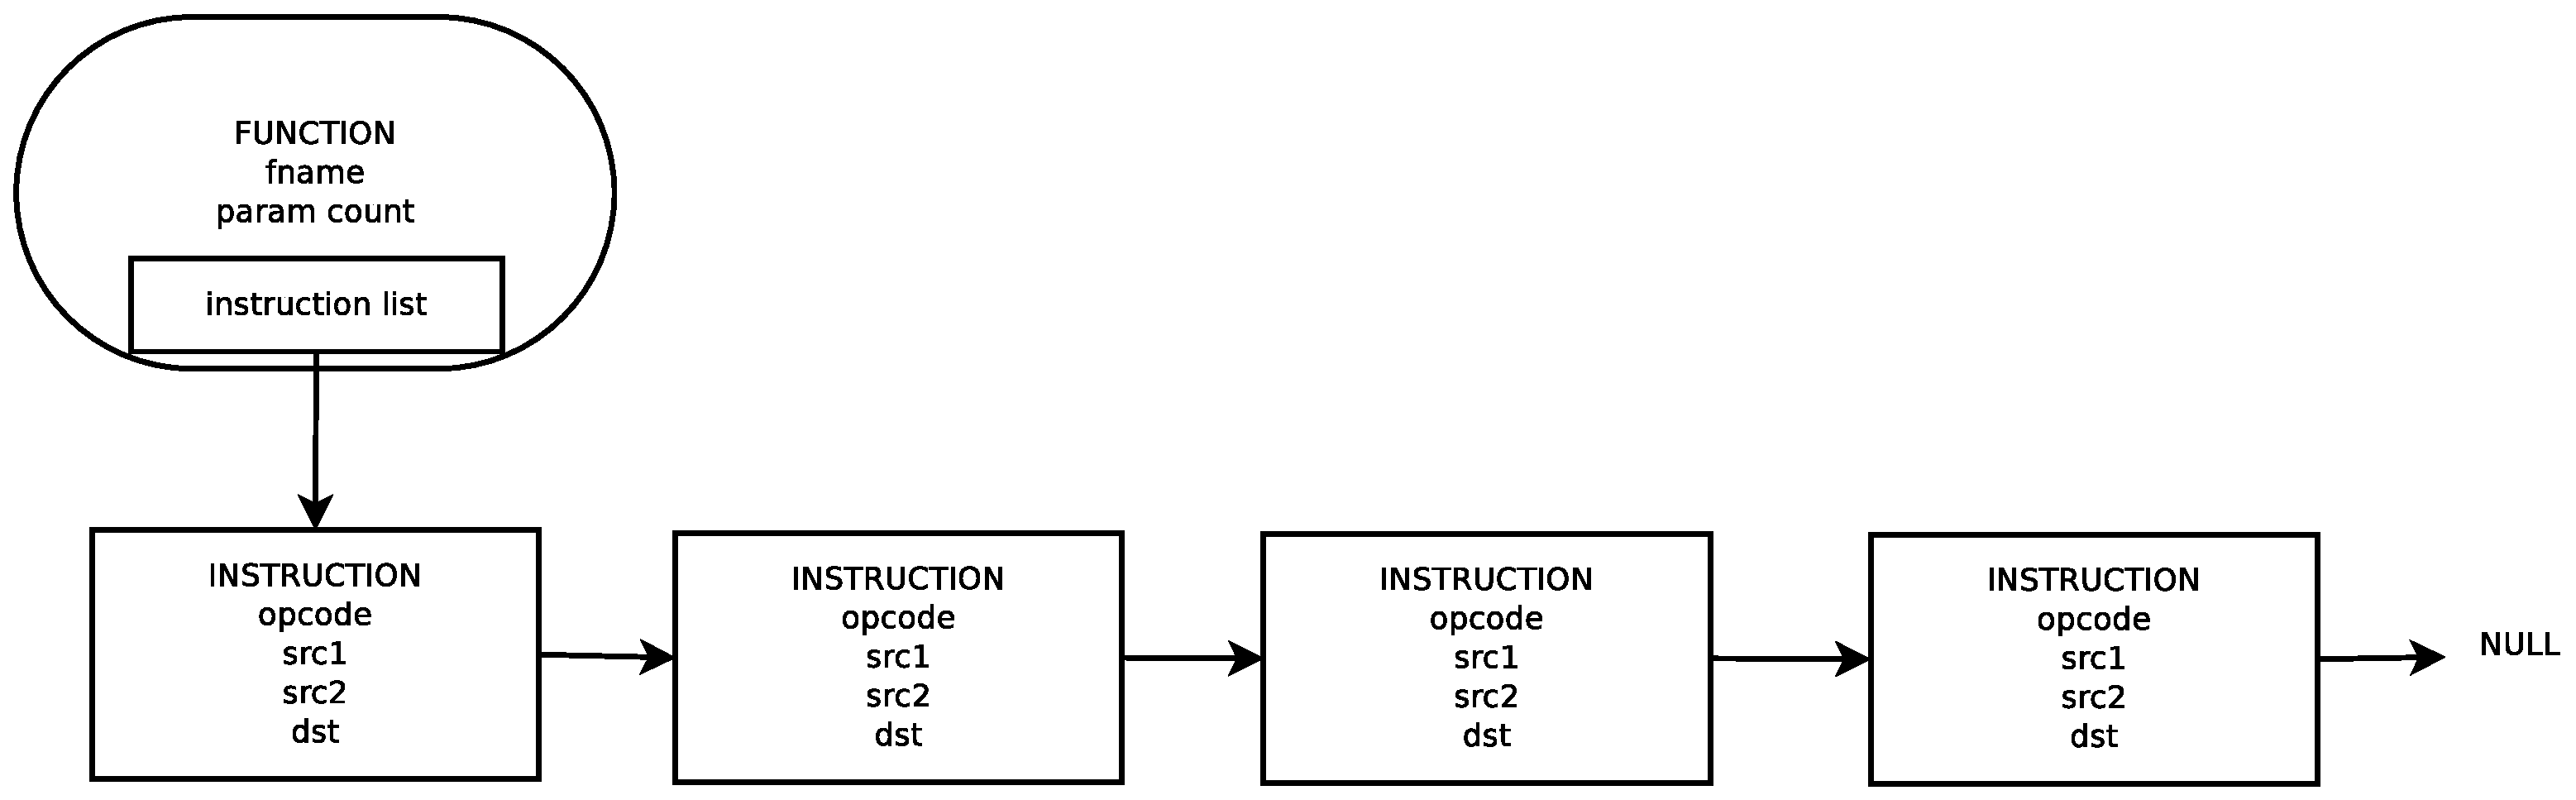
\includegraphics{img/instruction_list.eps}}
        \caption{Lineárny zoznam inštrukcií.}
        \label{int-obr1}
    \end{center}
\end{figure}

Interpret detekuje chyby, ktoré sa vyskytnú až za behu programu (príkladom môže
byť delenie nulou).

Operandom inštrukcie môže byť položka v~tabuľke symbolov (inštrukcia
\texttt{enter}, ktorá vytvára zálohu), premenná alebo inštrukcia
v~závislosti od sémantiky inštrukcie.

V~niektorých prípadoch semantická analýza prenecháva kontrolu typov operandov
pre interpret z~dôvodu jednoduchosti. Dochádza k~tomu hlavne pri premenných,
ktorým hodnota je priradená vstavaným príkazom \texttt{read}. Preto
interpret detekuje takéto chybné stavy pri aritmetických operáciach ako aj
operáciach porovnánia.  Interpret ďalej detekuje chybu pri práci
s~nepovolenými hodnotami premenných interne typovaných na \texttt{double} -
pretečenie na \texttt{NAN} a~\texttt{INFINITY}, \texttt{-INFINITY}.
\footnote{Definované v~štandardnom hlavičkovom súbore \texttt{float.h}}.

\begin{figure}[h]
    \begin{center}
        \scalebox{0.25}{\includegraphics{img/call_stack.eps}}
        \caption{Programový zásobník.}
        \label{int-obr2}
    \end{center}
\end{figure}

Inštrukcia \texttt{substr} je zvláštna svojím vyhodnocovaním. Ako jediná
z~inštrukčnej sady prepisuje zdrojový operand, ktorý je zároveň cieľovým
operandom. Je tak z~dôvodu, že vstavaná funkcia má tri parametre. Pre jednoduchú
implementáciu bola navrhnutá inštrukcia \texttt{substr}, ktorá je taktiež
trojadresná, no výsledok operácie je zapísaný do cieľového operandu, v~ktorom je
predaný reťazec. Preto sa výnimočne v~tomto prípade vygeneruje dodatočná
inštrukcia, ktorá vytvorí kópiu prvého parametru vstavanej funkcie
\texttt{substr} a~vloží ho do tabuľky symbolov. Táto kópia môže byť následne
prepísaná bez prípadnej straty dát.

Narozdiel od vstavanej funkcie \texttt{substr} je vstavaný príkaz \texttt{write}
zvláštny svojím počtom parametrov. Zjednodušenie implementácie viedlo k~tomu, že
bola navrhnutá jednoduchá inštrukcia \texttt{write}, ktorá vypisuje práve jeden
parameter. Pokiaľ bol vstavaný príkaz volaný s~viacero parametrami, vygeneruje
sa samostatná inštrukcia \texttt{write} pre každý parameter.

Inštrukcia \texttt{leave} je určená pre návrat z~funkcie definovanej užívateľom.
Inštrukcia \texttt{leave} je automaticky vkladaná na koniec funkcie a~za príkaz
\texttt{return}.  To spôsobí korektný návrat z~podprogramu.

\subsection{Voľba datových typov}

Interpret jazyka IFJ11 nie je typovým jazykom. Avšak interpret je písaný
v~jazyku C, ktorý je typovým jazykom, preto je nutné interne určovať datový typ,
ktorý aktuálne nadobúda premenná. Pre typ \texttt{string} je použitý
ukazateľ na pole \texttt{char}, pre typ \texttt{bool} je použitá premenná
typu \texttt{\_Bool}, pre čísla typ \texttt{double} \footnote{Číslo
s~plávajúcou desatinnou čiarkou s~dvojitou presnosťou podľa štandardu
ISO-IEEE 754.}. Typ \texttt{double} je vhodný pre svoj rozsah
a~presnosť, ktorá je požadovaná. Špeciálnym prípadom je typ
\texttt{nil}, ktorý nenadobúda žiadnu hodnotu.

Pre prácu s~premennými bol vytvorený abstraktný datový typ\,--\,štruktúra
\texttt{Tvariable}, ktorú možno nájsť v~hlavičkovom súbore \texttt{variable.h}.
Táto štruktúra zapuzdruje všetky spomínané typy, ktoré podporuje jazyk IFJ11.

V~lexikálnom analyzátore bol použitý abstraktný datový typ \texttt{string},
ktorý je definovaný v~súboroch \texttt{str.h} a~\texttt{str.c}. Ako základ
bol použitý vzorový interpret jednoduchého jazyka zo stránok predmetu IFJ,
ktorého autorom je Ing. Roman Lukáš PhD. Zdrojové súbory boli upravené pre
použitie v~interpretri IFJ11 (najmä pomenovanie metód/funkcií nad
abstraktným datovým typom).

\subsection{Volanie podprogramu a~návrat}

Imperatívny jazyk IFJ11 podporuje definovanie užívateľských funkcií
s~parametrami, ich volanie a~následný návrat na miesto volania. Pre tento
požiadavok boli navhnuté inštrukcie \texttt{enter}, \texttt{call}
a~\texttt{leave}.

Inštrukcia \texttt{enter} je prologom pred samotným volaním podprogramu. V~dobe
interpretácie je touto inštrukciou interpret informovaný, že nastane volanie
podprogramu. Parametrom inštrukcie je odkaz do tabuľky symbolov na položku
reprezentujúcu volajúcu funkciu. Interpret následne môže zahájiť tvorbu
aktivačného záznamu na programovom zásobníku. Skopíruje hodnoty a~typy všetkých
premenných a~vytvorí tak kópiu aktuálneho stavu premenných do zinicializovanej
položky na programovom zásobníku. Nasleduje sled inštrukcií \texttt{mov}
a~\texttt{clr}.

Po vykonaní inštrukcie \texttt{enter} nastáva predávanie parametrov.
Vygenerované inštrukcie predávajú hodnoty premenných priamo do zoznamu
premenných odkazovaných z~položky v~tabuľke symbolov (inštrukcie \texttt{mov})
prípadne ich nulujú (inštrukciou \texttt{clr}) v~prípade neuvedenenia
dostatočného počtu.

Prípravu volania podprogramu ukončuje inštrukcia \texttt{call}, ktorá na vrchol
programového zásobníka uloží adresu nasledovnej inštrukcie, ktorá bude vykonaná
po návrate z~podprogramu. Nasleduje vykonávanie prvej inštrukcie podprogramu.

Každá funkcia musí obsahovať aspoň jednu inštrukciu \texttt{leave}.  Inštrukcia
\texttt{leave} sa generuje na úplnom konci funkcie a~po príkaze \texttt{return},
ktorý najprv predá návratovú hodnotu. Pri interpretácii inštrukcie
\texttt{leave} sa obnoví záloha premenných funkcie, do ktorej sa podprogram
vracia a~zruší položky na vrchole zásobnika. Inštrukcia \texttt{leave} je
preto komplementárna s~inštrukciou \texttt{enter} a~je epilogom pri volaní
funkcie.


%%%%%%%%%%%%%%%%%%%%%%%%%%%%%%%%%%%%%%%%%%%%%%%%%%%%%%%%%%%%%%%%%%%%%%%%%%%%%%%%

\section{Záver} \label{zaver}
Projekt IFJ11 bol naším prvým tímovým projektom. Počas jeho tvorby sme si
rozšírili svoje znalosti a~získali skúsenosti s~prácou na rozsiahlejšom projekte
a~prácou v~tíme. Spoznali sme náročnosť rôznych fáz tvorby projektu od návrhu až
po testovanie. Využili sme pokusné odovzdanie, ktoré nám pomohlo získať
predstavu o~stave jednotlivých častí projektu, vďaka čomu sme sa vedeli zamerať
na slabšie miesta našej implementácie. Projekt hodnotíme veľmi pozitívne.
Nadobudnuté znalosti uplatníme v~profesionálnej kariére.

%Bibliograficke citacie
%%%%%%%%%%%%%%%%%%%%%%%%%%%%%%%%%%%%%%%%%%%%%%%%%%%%%%%%%%%%%%%%%%%%%%%%%%%%%%
\addcontentsline{toc}{section}{Literatúra} %prida polozku do obsahu
\bibliographystyle{czplain}
\bibliography{literatura}

%Priloha
%%%%%%%%%%%%%%%%%%%%%%%%%%%%%%%%%%%%%%%%%%%%%%%%%%%%%%%%%%%%%%%%%%%%%%%%%%%%%%
\appendix
\section{Metriký kódu}
     \paragraph{Počet súborov:} 30 súborov
     \paragraph{Počet riadkov zdrojového kódu:} 9378 riadkov
     \paragraph{Veľkosť statických dát:} 968B
     \paragraph{Veľkosť spustiteľného súboru:} 52kB (systém GNU/Linux,
                64 bitová architektúra, pri preklade bez ladiacich informácií)

\begin{figure}[h!]
    \section{Štruktúra konečného automatu lexikálneho analyzátora} \label{obr-lex}
    \begin{center}
        \scalebox{0.5}{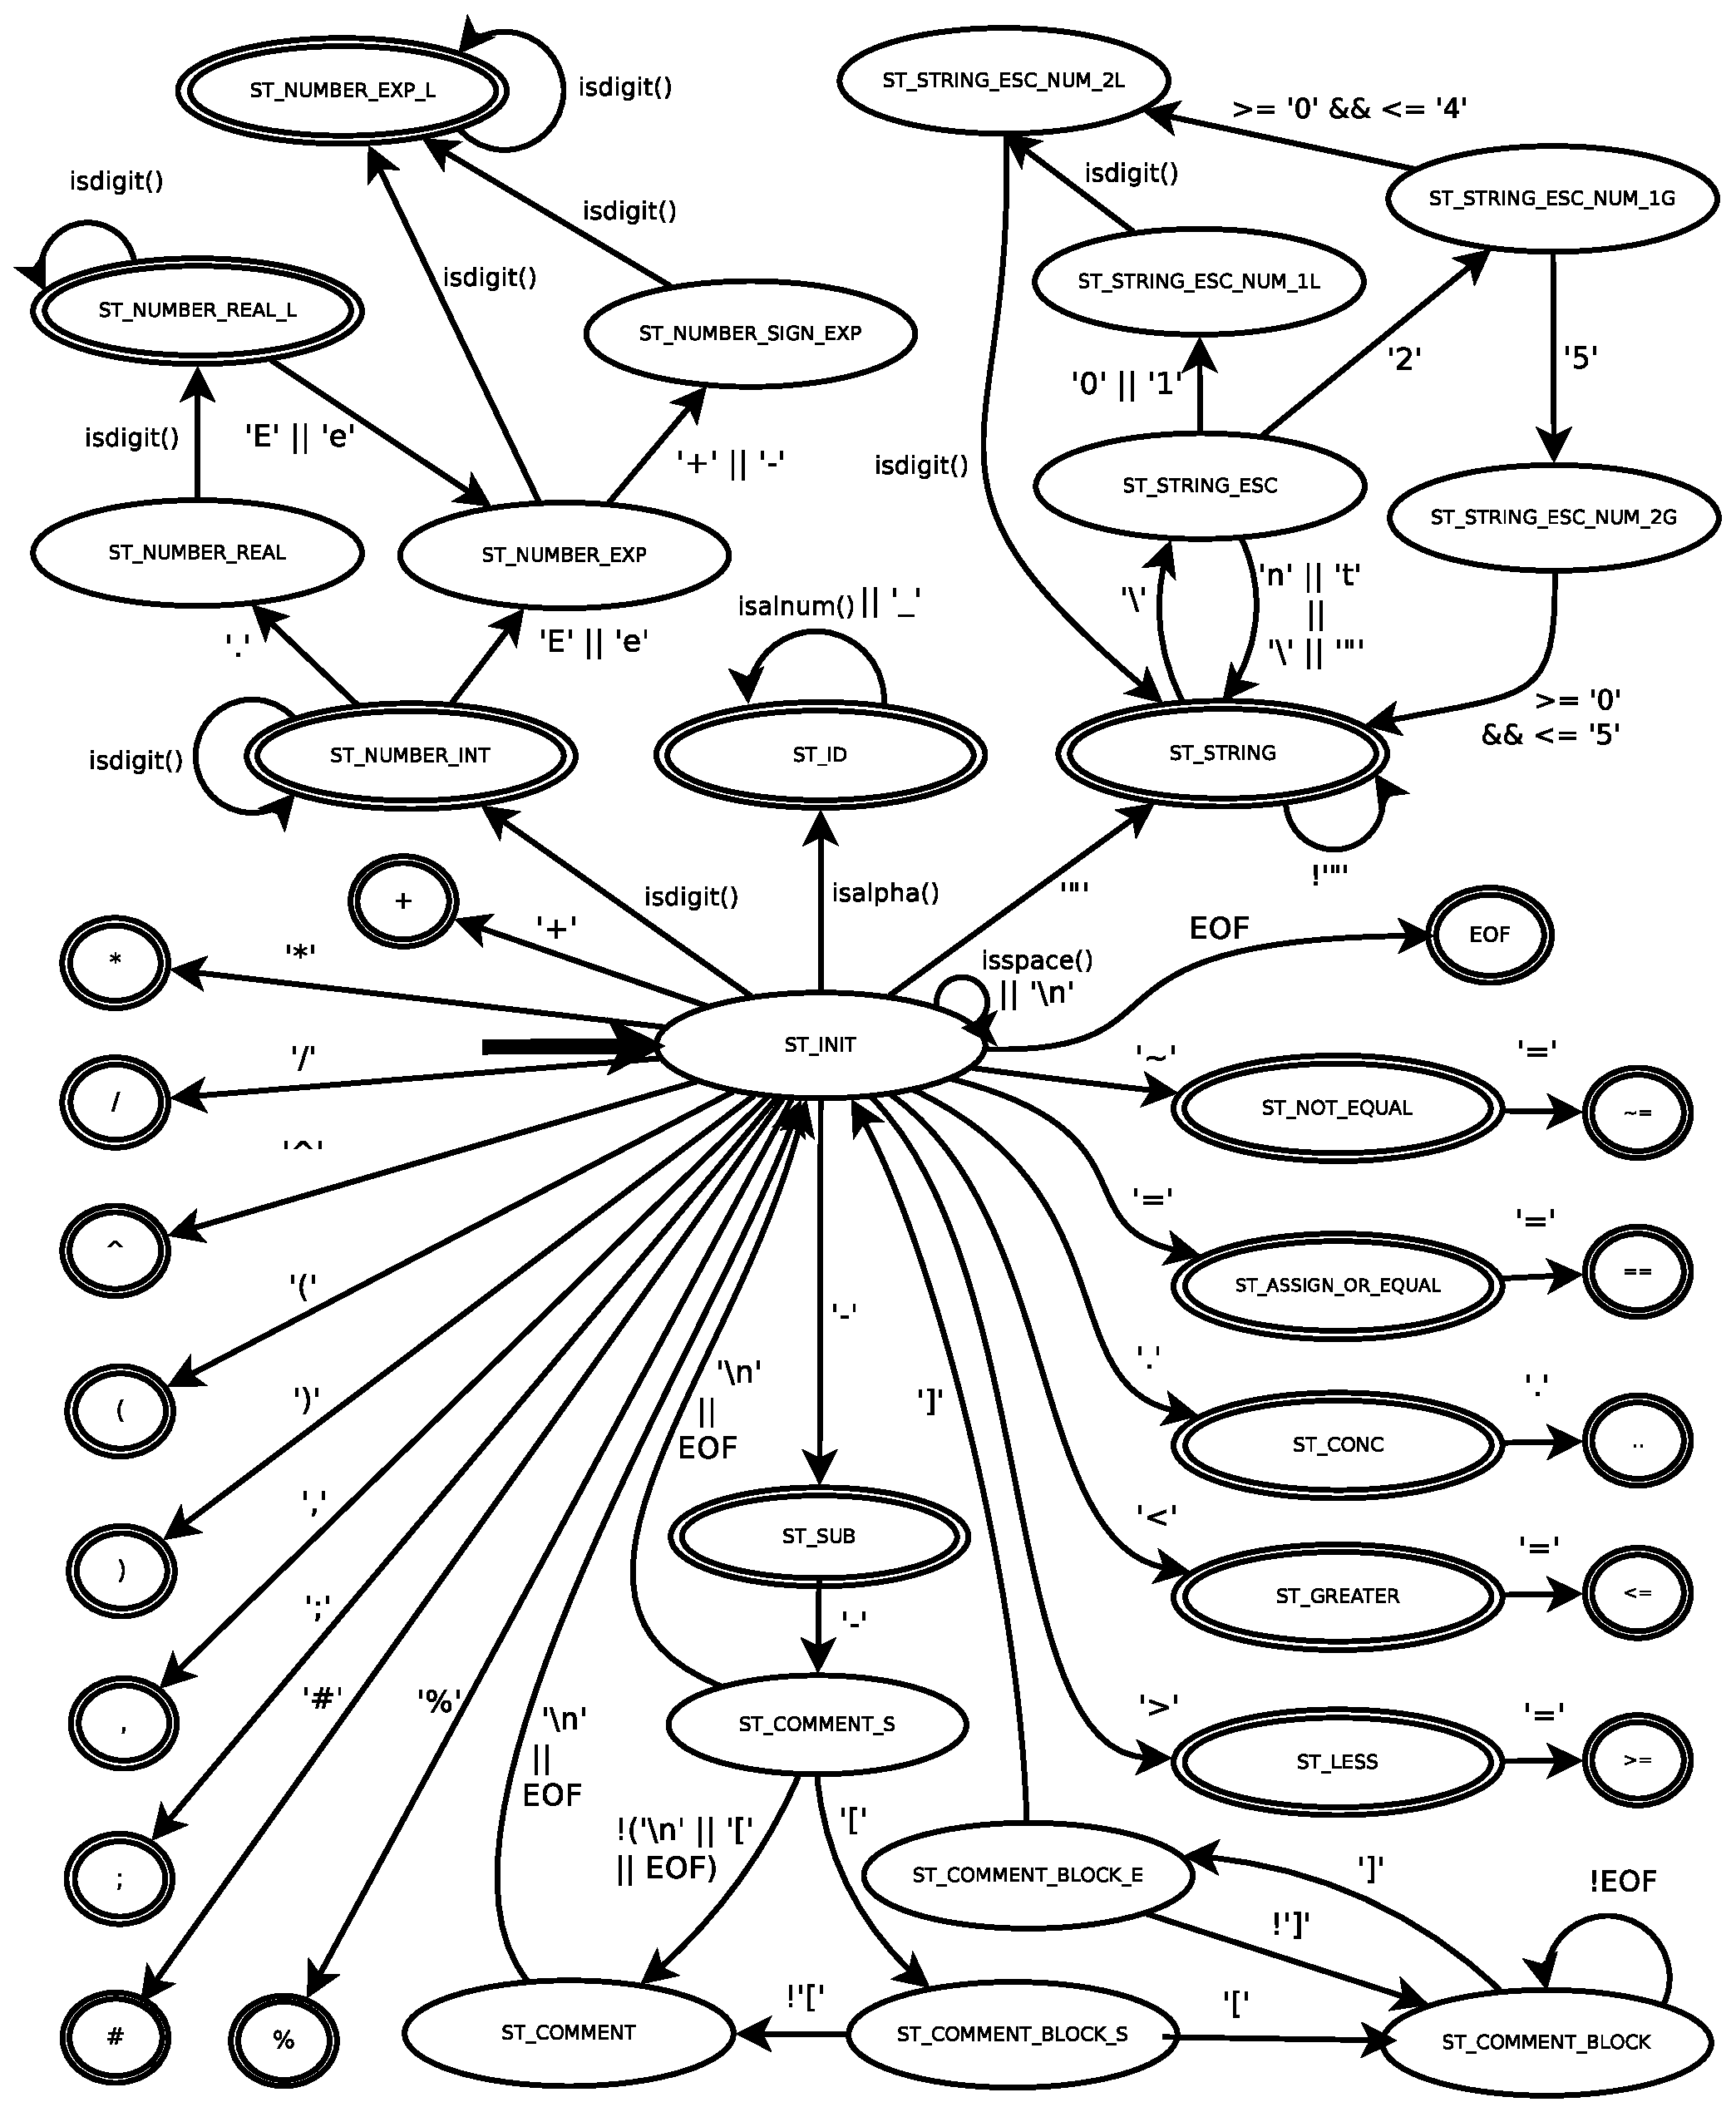
\includegraphics{img/scanner.eps}}
    \end{center}
    \caption{Konečný automat lexikálneho analyzátora}
\end{figure}


\begin{table}[h!]
    \section{Tabuľka pravidiel LL-gramatiky} \label{tabulka_pravidiel_ll_gramatiky}
    \begin{tabular}{llll}
        1. & \textless prog\textgreater & $ \rightarrow $ & \textless
        df-list\textgreater \,EOF\\
        2. & \textless df-list\textgreater & $ \rightarrow $ & FUNCTION ID (
        \textless param-list\textgreater \,\textless var-list\textgreater\\
        3. & \textless param-list\textgreater & $ \rightarrow $ & )\\
        4. & \textless param-list\textgreater & $ \rightarrow $ & ID \textless
        param\textgreater\\
        5. & \textless param\textgreater & $ \rightarrow $ & , ID \textless
        param\textgreater\\
        6. & \textless param\textgreater & $ \rightarrow $ & )\\
        7. & \textless var-list\textgreater & $ \rightarrow $ & LOCAL ID
        \textless dclr-type\textgreater \,\textless var-list\textgreater\\
        8. & \textless var-list\textgreater & $ \rightarrow $ & \textless
        stat-list\textgreater\\
        9. & \textless dclr-type\textgreater & $ \rightarrow $ & ;\\
        10. & \textless dclr-type\textgreater & $ \rightarrow $ & = \textless
        expr\textgreater \, ;\\
        11. & \textless stat-list\textgreater & $ \rightarrow $ & \textless stat
        \textgreater \, ; \textless stat-list\textgreater\\
        12. & \textless stat-list\textgreater & $ \rightarrow $ & END \textless
        end\textgreater\\
        13. & \textless stat\textgreater & $ \rightarrow $ & ID \textless
        id-or-fun\textgreater\\
        14. & \textless stat\textgreater & $ \rightarrow $ & WRITE ( \textless
        w-args-list\textgreater\\
        15. & \textless stat\textgreater & $ \rightarrow $ & RETURN \textless
        expr\textgreater\\
        16. & \textless stat\textgreater & $ \rightarrow $ & WHILE \textless
        expr\textgreater \, DO \textless stat-list\textgreater\\
        17. & \textless stat\textgreater & $ \rightarrow $ & REPEAT \textless
        stat-repeat-list\textgreater \, \textless expr\textgreater\\
        18. & \textless stat\textgreater & $ \rightarrow $ & IF \textless expr
        \textgreater \, THEN \textless stat-if-list\textgreater\\
        19. & \textless end\textgreater & $ \rightarrow $ & ;\\
        20. & \textless end\textgreater & $ \rightarrow $ & \textless df-list
        \textgreater\\
        21. & \textless stat-repeat-list\textgreater & $ \rightarrow $ & UNTIL\\
        22. & \textless stat-repeat-list\textgreater & $ \rightarrow $ &
        \textless stat\textgreater \, ; \textless stat-repeat-list\textgreater\\
        23. & \textless stat-if-list\textgreater & $ \rightarrow $ & \textless
        stat\textgreater \, ; \textless stat-if-list\textgreater\\
        24. & \textless stat-if-list\textgreater & $ \rightarrow $ & ELSE
        \textless stat-list\textgreater\\
        25. & \textless stat-if-list\textgreater & $ \rightarrow $ & ELSEIF
        \textless stat-if-list\textgreater\\
        26. & \textless stat-if-list\textgreater & $ \rightarrow $ & END
        \textless end\textgreater\\
        27. & \textless id-or-fun\textgreater & $ \rightarrow $ & = \textless
        rfe\textgreater\\
        28. & \textless id-or-fun\textgreater & $ \rightarrow $ & ( \textless
        args-list\textgreater\\
        29. & \textless w-args-list\textgreater & $ \rightarrow $ & \textless
        expr\textgreater \, \textless w-arg\textgreater\\
        30. & \textless w-arg\textgreater & $ \rightarrow $ & , \textless expr
        \textgreater \, \textless w-arg\textgreater\\
        31. & \textless w-arg\textgreater & $ \rightarrow $ & )\\
        32. & \textless rfe\textgreater & $ \rightarrow $ & READ ( \textless
        read-format\textgreater \, )\\
        33. & \textless rfe\textgreater & $ \rightarrow $ & ID \textless fe
        \textgreater\\
        34. & \textless fe\textgreater & $ \rightarrow $ & \textless expr
        \textgreater\\
        35. & \textless fe\textgreater & $ \rightarrow $ & ( \textless
        args-list\textgreater\\
        36. & \textless args-list\textgreater & $ \rightarrow $ & )\\
        37. & \textless args-list\textgreater & $ \rightarrow $ & \textless
        lit-or-id\textgreater \, \textless arg\textgreater\\
        38. & \textless arg\textgreater & $ \rightarrow $ & , \textless
        lit-or-id\textgreater \, \textless arg\textgreater\\
        39. & \textless arg\textgreater & $ \rightarrow $ & )\\
        40. & \textless lit-or-id\textgreater & $ \rightarrow $ & ID\\
        41. & \textless lit-or-id\textgreater & $ \rightarrow $ & NUMBER\\
        42. & \textless lit-or-id\textgreater & $ \rightarrow $ & STRING\\
        43. & \textless lit-or-id\textgreater & $ \rightarrow $ & FALSE\\
        44. & \textless lit-or-id\textgreater & $ \rightarrow $ & TRUE\\
        45. & \textless lit-or-id\textgreater & $ \rightarrow $ & NIL\\
        46. & \textless read-format\textgreater & $ \rightarrow $ & NUMBER\\
        47. & \textless read-format\textgreater & $ \rightarrow $ & STRING\\
        48. & \textless expr\textgreater & $ \rightarrow $ & PSA\\
    \end{tabular}
    \caption{Tabuľka pravidiel LL-gramatiky}
\end{table}
\end{document}

